%----------------------------------------------------------------------------------------
%	Software
%----------------------------------------------------------------------------------------

\chapter{Software Components}

The software requirements of this project include embedded software, a backend and two frontends. The embedded software will communicate with the hardware and the software backend. The backend will store data and communicate with the frontends, which will display the information to SPCA staff and allow them to enter weights. This section will review existing products and specify our software design. 

\section{Prior Art}

In this section, existing software solutions for smart scales are discussed and compared.

PitPat is an app and activity tracker for dogs that provides various features to help dog owners monitor their pet's fitness and well-being. The technical specifications include bluetooth connectivity, data analysis using complex algorithms to analyse the data collected by the PitPat monitor, and cloud-based storage. Some functional specifications are dog activity tracking, daily goals, health and fitness insights, and personalised recommendations based on your dog's activity levels and other information.

This app tracks your pet's weight, exercise, food intake, and other health metrics. It also offers customised diet plans and reminders for vet appointments. The technical specifications include WiFi connectivity, automatic updates, and smart notifications. Some functional specifications are weight tracking, diet and nutrition tracking, exercise tracking, medication reminders, and breed information.
Petable is a pet health and wellness app that provides various features to help pet owners manage their pet's health and well-being. The technical specifications include cloud-based storage, AI, secure data protection, and multi-platform compatibility. Some functional specifications are health and nutritional tracking based on breed, diet and feeding schedule.

Overall, there does not seem to be any applications specifically for keeping track of animal weights. The applications found are all related to pet health where tracking the weight of the animal is part of the application’s functionality, but not the main focus.


\section{Embedded}
The first step for the embedded section starts with the communication between the PCB and the Raspberry Pi. We are measuring the voltage of the output signal generated by the instrumentation amplifier to give us an indication of the weight present on the scale. We will also measure the voltage value of the PCB ground on a separate ADC channel, this will allow us to measure the inherent offset in the Pi’s ADC. We can then write firmware to convert the ADC values into weights as the circuitry has been designed to vary the output voltage linearly with weight. 

The measured weight will be the average of multiple samples. The scale should stop measuring once the weight has stabilised within a certain range. Then it will take an average of the samples measured and take that as the weight of the dog. The specifics of the algorithm will be developed through practical testing on a working prototype. 

Once we have these voltages, we can send them to the backend of the website and app via a POST request over HTTP or HTTPS. 

The workflow for the communication between the Raspberry Pi and the backend is that every time a dog is weighed, the measurements and a scale ID are sent to the backend.The backend will always store the most recent value sent from each scale, but at this stage it is not associated with any dog. Once the user is happy with measurement, they can take the most recent weight and link it with a dog ID to store it in the dog database.

We have decided to include a seven-segment display into our design. This is done for the purpose of convenience and reliability. It increases convenience as the user can immediately read the weights without needing to interact with the system. It also adds reliability as the scale would be able to function without wifi, which may occur for several reasons. Many people may not be proficient with technology and prefer a more manual workflow which will require some sort of display. 


\section{Backend}

For the backend, we have used .NET with C\# for the Web API endpoints, integrated with a light weight SQLite serverless database for data handling. For data tracking, we are planning to have: user login information, centre information, animal information, and chat messages. The information will be stored in a few SQL tables in the database. (Refer to Figure \ref{fig:database-1} in Appendix C).

The backend web API will work with the database to carry out Create, Read, Update, and Delete operations in order to satisfy the business requirements from the SPCA.

We will have API endpoints for user, dog, and chat operations. Some user operation endpoints include things such as authentication, registration, and managing existing users. Dog operations include adding, editing, and deleting dogs. Other dog endpoints include viewing dog information from different SPCA centres and triggering alerts for weight. Finally, chat operations include sending messages to other users of the application as well as retrieving one’s own chat history. Each endpoint requires a specific level of access rights so that users are only authorised to use the endpoints that they are allowed to use.

Most of the endpoints will be secured with Basic Authentication that is configurable as part of the .NET framework. This means Authentication header for HTTP requests will be needed to access most of the secured API endpoints. Username and Password combination as an encoded string will be sent over the secure HTTPS network to eliminate the chance of being compromised. On the other hand, Basic Authentication will support the distinction of different user types, therefore, we can further secure the access level of different users on the API, not only from the front end of the application, in order to minimise the chance for API endpoints to be abused. For the single endpoint of hardware access for sending over weight data, it is not secured due to the added complexity of implementing it. However, we will add a pseudo password string so any request coming through this API that does not contain this string will be ignored.


\section{Frontends}
We have decided to create two front-end frameworks: a mobile application built in Android Studio, and a web application built in React JS. Both applications will have the same functionality so that users can easily switch between both platforms, however we will not support real-time updates. Creating a mobile application is ideal for vets and volunteers to use while they are on the go, and they can easily record dogs weight with the scales wherever they are. The web application will be helpful for administrators to track trends across centres, and export data to use in excel and other workflows. 

We will supply some key functionalities to our users. They will be able to log in and out of their account and change their password. Admins can view dogs across all centres, whereas vets and volunteers are restricted to the centre that they work in. Users can create dogs, view dogs’ history, and add a new weight. Dogs can be ‘flagged’ or set on ‘alert’, indicating that they need to be weighed, or that they are experiencing alarming weight change. Users can view trends across dogs and centres, send messages to other users, and admins can edit the users’ access. 

Below is a look at the UI of the mobile application. The web application can be seen in Figure \ref{fig:webapp-1} Appendix D. The user can navigate through the main screens by the navigation bar on the bottom, and the red arrows show navigation to additional screens.
\begin{figure}[!ht]
	\centering
	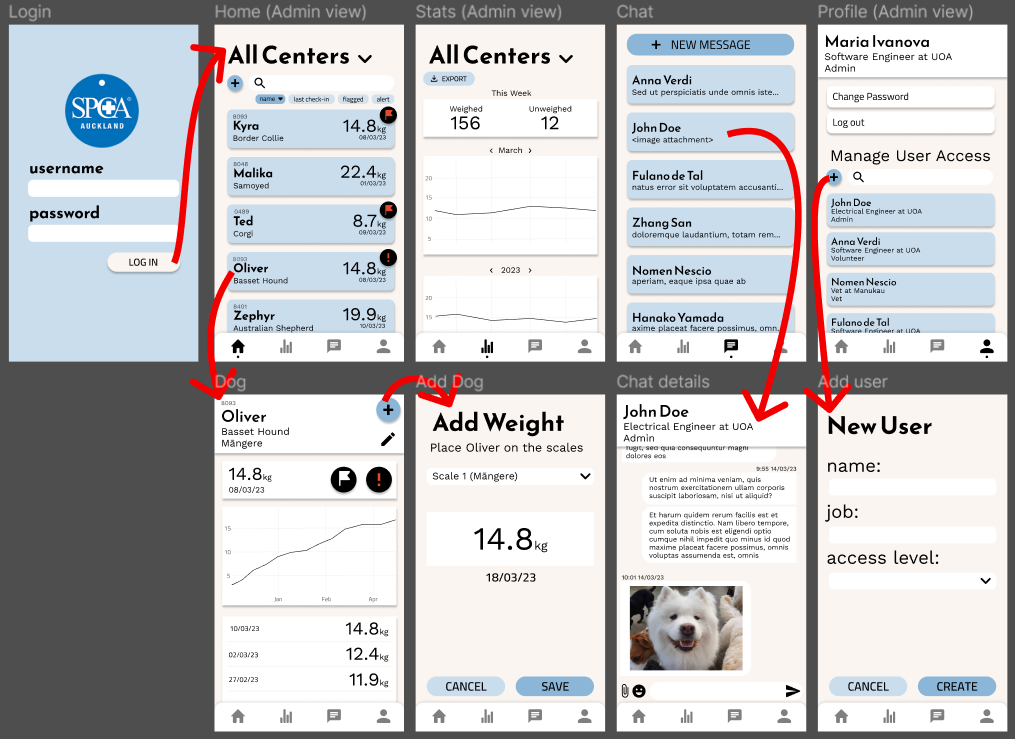
\includegraphics[scale=0.3]{sw-mobile-app-ui.png}
	\caption{Mobile UI High-fidelity Prototype.}
	\label{fig:mobileapp-1}
\end{figure}

 

